\section{Conjunto de Dados e Metodologia}

% Responsável pelo Dataset: Dev 1
\subsection{Conjunto de dados}

Foi usado o conjunto \emph{Human Activity Recognition Using Smartphones} \cite{anguita2013,uci_har}. Trinta voluntários, entre 19 e 48 anos, realizaram seis atividades carregando um smartphone preso à cintura: caminhar, subir escadas, descer escadas, sentar, ficar em pé e deitar. O acelerômetro e o giroscópio foram amostrados a 50~Hz, e os sinais foram divididos em janelas de 2,56~s com 50\% de sobreposição. Os dados são medidas numéricas dos sensores; os vídeos foram usados pelos autores originais apenas para anotar as atividades.

Cada janela é descrita por 561 características calculadas nos domínios do tempo e da frequência, normalizadas para o intervalo $[-1, 1]$. O conjunto totaliza 10.299 janelas e traz a divisão oficial em treino, com 7.352 janelas de 21 participantes, e teste, com 2.947 janelas de 9 participantes diferentes. Essa divisão foi mantida. A identificação do participante é usada somente para separar e validar os dados, nunca como entrada dos modelos.

A análise exploratória (Tabela~\ref{tab:splits} e Figura~\ref{fig:classes}) mostrou que as classes são razoavelmente equilibradas, entre 13\% e 19\% das janelas, e que todos os participantes têm exemplos das seis atividades, com 281 a 409 janelas cada. Não há valores ausentes, linhas repetidas nem características constantes.

\begin{table}[t]
  \caption{Divisão oficial do conjunto de dados.}
  \label{tab:splits}
  \centering
  \begin{tabular}{lrrr}
    \toprule
    Partição & Janelas & Participantes & Características \\
    \midrule
    Treino & 7.352 & 21 & 561 \\
    Teste  & 2.947 & 9  & 561 \\
    \bottomrule
  \end{tabular}
\end{table}

\begin{figure}[t]
  \centering
  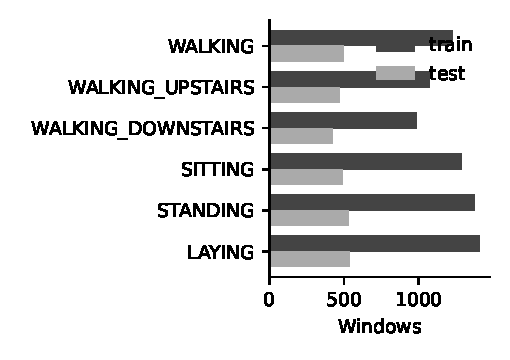
\includegraphics[width=\columnwidth]{figures/class_distribution.pdf}
  \caption{Janelas por atividade nas partições de treino e teste.}
  \label{fig:classes}
\end{figure}

% Responsável pela Metodologia: Dev 2 (validação agrupada, métricas, semente e versões).
\subsection{Metodologia}
